%!TEX root = main.tex
% Legger alt av usability stuff her enn så lenge

% Bruk testplan.docx og test-report.docx som en slags mal til hva som skal være med i plan og rapport. Legg det inn her 
% Se på Usability Master 2 Svanaes.pdf for et forslag til oppsett av dette. F.eks en section med gjennomføring og en med resultater. Slå sammen stuffet fra testplan.docx og test-report.docx til en fin ting!  
\chapter{Usability}
% Her bør vel det nevnes det fra testplanen, kjapt hva vi ville og resultatene stå. Vi bør også forklare testplanen mer et annet sted, såvidt i research method? Men kanskje også reintrodusere test-kapitlet og legge alt fra intro til resultater der? Bør vel ikke stå altfor mye i intro kapitlet dog
% Usability testen er jo ikke den primære evalueringen, men iom. at vi har begrenset med data bør vi nok fokusere litt på den. 
In this section we will describe the results and observations gained through usability tests. Before we conducted the usability test we created a usability test plan: Appendix \ref{chap:usability}, where all the different parts of the usability test is described in detail.

The usability test was conducted on four participants. User-interaction with the PeacefulBanana was done through an Internet Browser. Users answered an entrance questionnaire, in order to collect demographic information. During the usability test we took notes of the user's problems and concerns. When the test was completed, participants could comment with suggestions on improvement of the application or design. Finally we had participants answer a SUS form, which consisted of 10 questions designed to measure user satisfaction. 

\subsection{Context}
\label{subsec:context}
The usability test simulated the two scenarios identified in Section \ref{sec:scenarios} and was set in the context of these. We conducted the usability test in order to answer several important questions, regarding these scenarios: 
\begin{itemize}
	\item Is the application easy to use, and can users achieve their goals in a timely manner?
	\item Identify the relationship users have with the aspect of reflection and sharing personal experiences.
	\item Does the tool present data in a way that triggers reflection for the user?
\end{itemize}
Feedback from the usability test was used to further aid design and help identify problem areas that might cause problems for potential users. Since the participants were all computer science experts, and familiar with reflection we hoped to collect valuable input regarding these concepts.

\subsection{Participants}
As mentioned we had four participants in the usability test. As the PeacefulBanana tool is intended to be used with developers with a computer-science background, participants were master students on the Computer Science field at NTNU. These participants all had a background from Computer Science, and were familiar with usability testing and also experienced with the notion of reflection from earlier projects using agile methodologies.
The participants' responsibilities were to attempt to complete a set of representative task scenarios presented to them in as efficient and timely a manner as possible, and to provide feedback regarding the usability and acceptability of the user interface. The participants was directed to provide honest opinions regarding the usability of the application, and to participate in post-session subjective questionnaires and debriefing.

\subsection{Procedure}
The usability test took place in a private room at the university. A computer with the PeacefulBanana web application was used in a typical working environment. The participants interaction with the application was monitored by the facilitator seated in the same room.
The facilitator briefed the participants on the web application and instructed the participants that are evaluating the application, rather than evaluating the participant. Participants signed an informed consent that acknowledges: \emph{the participation is voluntary, that participation can cease at any time, and that their privacy of identification will be kept safe}. \\
The facilitator explained that the amount of time taken to complete the test task will be measured and that exploratory behavior outside the task flow should not occur until after task completion. At the start of each task, the participant read aloud the task description from the printed copy and began the task. Time-on-task measurement began when the participant started the task.
The facilitator instructed the participant to ‘think aloud’ so that the facilitator could observe and take notes of user behavior and user comments.
After all task scenarios are attempted, the participant completed the post-test satisfaction questionnaire.

\subsection{Roles}
For our usability test we had two roles, in addition to the test participants:
\subsubsection{Facilitator}
	\begin{itemize}
		\item Provides overview of study to participants.
		\item Defines usability and purpose of usability testing.
		\item Responds to participant's requests for assistance.
	\end{itemize}
\subsubsection{Test Observer}
	\begin{itemize}
		\item Silent observer
		\item Takes notes of identified problems, concerns, coding bugs, and procedural errors.
		\item Serve as note takers.
	\end{itemize}

\subsection{Ethics}
All persons involved with the usability test were required to adhere to the following ethical guidelines:
\begin{itemize}
	\item The performance of any test participant must not be individually attributable. Individual participant's name should not be used in reference outside the testing session.
	\item A description of the participant's performance should not be reported. 
\end{itemize}

\subsection{Usability Tasks}
The usability tasks were derived from our scenarios, described in section \ref{sec:scenarios}. Due to the short time for which each participant was available, the tasks used were the most common and relatively complex of available functions. The tasks were identical for all participants in the study.
The application was tested in a development environment and databases were populated during use, and not pre-populated. This ensured a similar experience as to what the users would get when they first use PeacefulBanana in a real-life setting. The web application was run on a local computer, and not on a dedicated server as it was when deployed in production. This and the possible extra overhead from development mode, may have an impact on performance slightly in a negative way.

\subsubsection{Task context}
PeacefulBanana is a tool intended to promote reflection and allow for revisiting and learning from previous experiences. PeacefulBanana integrates with and collects data from the version-control system GitHub.
\subsubsection{Scenario 1 tasks:}
Here are the tasks participants were to solve related to Scenario 1:
\begin{itemize}
	\item Task 1: You start the application for the first time, and want to login, link your account with Github and set an active repository.
	\item Task 2: 
		\begin{itemize}
			\item Task 2.1: View your notifications.
			\item Task 2.2: Find the \emph{“Congratulations”} notification and archive it. Find the archive and see if the notification was indeed archived
		\end{itemize}
	\item Task 3:
		\begin{itemize}
			\item Task 3.1: Find the \emph{“Reminder: Daily Reflection”} note and perform the daily summary.
			\item Task 3.2: Find a daily summary note and share it. Verify that is has indeed been shared.
			\item Task 3.3: Find your mood graph
		\end{itemize}
\end{itemize}

\subsubsection{Scenario 2 tasks:}
Here are the tasks participants were to solve related to Scenario 2:
\begin{itemize}
\item Task 4:
	\begin{itemize}
		\item Task 4.1: Create a team with the name \emph{“Tuttifrutti”} and your previously chosen repository.
		\item Task 4.2: Find your created team and set it to active.
		\item Task 4.3: Identify the members on your team and their role.
	\end{itemize}
\item Task 5:
	\begin{itemize}
		\item Task 5.1: Find all your repositories’ milestones.
		\item Task 5.2: Identify your overdue milestones.
		\item Task 5.3: Find your repositories issues.
		\item Task 5.4: Find issue \#17 . Find the status of this issue, when it was opened and when it was closed.
	\end{itemize}
\item Task 6:
	\begin{itemize}
		\item Task 6.1: Generate a tagcloud for your current chosen repository.
		\item Task 6.2: Identify the most used tag for your team and yourself.
		\item Task 6.3: Find the commit impact for your repository.
	\end{itemize}
\end{itemize}

\subsection{Usability Metrics}
Usability metrics refers to user performance measured against specific performance goals necessary to satisfy usability requirements. Scenario completion success rates, error rates, and subjective evaluations was collected. Time-to-completion/Time-on-task was also collected.

\subsubsection{Task Completion}
Each task requires that the participant obtains or inputs specific data that would be used in course of a typical task. The task is noted as \emph{completed} when the participant indicates the task's goal has been obtained (whether successfully or unsuccessfully).  If a participant requires assistance in order to achieve a correct output then the task will be noted as a critical error and the overall completion rate for the task will be affected.

\subsubsection{Critical Errors}
A critical error is an error that results in an incorrect or incomplete outcome.. Obtaining or otherwise reporting of the wrong data value due to participant work flow is a critical error. Participants may or may not be aware that the task goal is incorrect or incomplete. In general, critical errors are unresolved errors during the process of completing the task or errors that produce an incorrect outcome.

\subsubsection{Non-Critical Errors}
Non-critical errors are errors that are recovered from by the participant or, if not detected, do not result in processing problems or unexpected results. Although non-critical errors can be undetected by the participant, when they are detected they are generally frustrating to the participant.

\subsubsection{Subjective Evaluations}
Subjective evaluations regarding ease of use and satisfaction was collected via questionnaires, and during debriefing at the conclusion of the session. The questionnaires utilized free-form responses and rating scales.

\subsubsection{Task Completion Time(time on task)}
The time to complete a task is referred to as "time on task", not including subjective evaluation duration. It is measured from the time the person begins the task to the time the participant indicates completion.

\subsection{Usability Goals}
The next section describes the usability goals for \emph{PeacefulBanana} in context of the usability metrics. First the general usability test objectives are described, and what usability metric results we aimed for.\\ 
The goals of usability testing the PeacefulBanana application included establishing a baseline of user performance, validating user performance measures, and identifying potential design issues that needed to be addressed in order to improve efficiency, usability and end-user satisfaction. \\
The general usability test objectives were:
\begin{itemize}
	\item Identify possible problems or breakdowns in the design\cite{ref:30} early on in the design process. Sources of such breakdowns may include:
		\begin{itemize}
			\item Navigation errors – failure to locate functions, excessive actions to complete a function, failure to follow recommended screen flow.
			\item Presentation errors – failure to locate and properly act upon desired information in screens, selection errors due to labeling ambiguities.
			\item Control usage problems – improper tool bar or entry field usage.
		\end{itemize}
	\item Exercise the PeacefulBanana application under controlled test conditions with representative users, which here are individuals with a background in IT. Data will be used to assess whether usability goals regarding an effective, efficient, and well-received user interface have been achieved.
	\item Establish baseline user performance and user-satisfaction levels of the user interface for future usability evaluations.
\end{itemize}
The PeacefulBanana application has been developed with developers in mind, and will be evaluated on students in the field of Computer Science, developing in an agile team. The testing will occur in a controlled environment in a private room.

Typical problems identified in a usability test would be text representations or the placement of design elements, that are not intuitive for the user during use. It would be a concern if the user can't figure out how to use certain features of the application. Identifying these problems as early as possible will lead to a better end design. \\
Secondly an objective of the usability test was to identify how users act and think about their daily experiences, how they react to the notion of reflecting on them and if sharing their private thoughts is a problem. 

\subsubsection{Completion Rate}
A completion rate of 100\% is the goal for each task in this usability test. \\
Completion rate is the percentage of test participants who successfully complete the task without critical errors, an \emph{output} that is correct. If a participant requires assistance in order to achieve a correct output then the task will be scored as a critical error and the overall completion rate for the task will be affected.

\subsubsection{Error-Free rate}
An error-free rate of 75\% is the goal for each task in this usability test. \\
Error-free rate is the percentage of test participants who complete the task without any errors (critical or non-critical errors). A non-critical error is an error that is not critical to get correct task output but would result in the task being completed less efficiently.

\subsubsection{Subjective Measures}
Opinions of participators regarding specific tasks, time to perform each task, features, and functionality was collected. At the end of the usability test, participants rated their satisfaction with the overall system. Combined with the interview/debriefing session. 

\subsection{Problem Severity}
In order to analyze collected data from the usability test, identified issues were classified by issue severity. This issue severity is a combination of the impact of the issue and the frequency of users experiencing the issue during the test. 

\subsubsection{Impact}
\subsubsection{Frequency}
	\begin{itemize}
		\item High: 40\% or more of the participants experienced the problem.
		\item Moderate: 20\% - 39\% of participants experienced the problem.
		\item Low: 20\% or fewer of the participants experienced the problem
	\end{itemize}
\subsubsection{Problem Severity Classification}
	\begin{itemize}
		\item High severity: High impact problems that often prevent a user from correctly completing a task. Reward for resolution is reduced redevelopment costs.
		\item Medium severity: Either moderate problems with low frequency or low problems with moderate frequency; these are minor annoyance problems faced by a number of participants. Reward for resolution is typically exhibited in reduced time on task and increased data
		\item Low severity: Low impact problems faced by few participants; there is low risk to not resolving these problems. Reward for resolution is typically exhibited in increased user satisfaction.
	\end{itemize}

\section{Usability Test Results}
\subsection{Pilot Test}
After finalizing the usability test plan: Appendix \ref{chap:usability}, a pilot test was conducted prior to the usability-test[ref 22]. The pilot test allows for an evaluation of the test plan itself and the questionnaires before doing the actual usability test. This means the pilot test is a "test of the test", where the goal is to evaluate and verify that the test itself is well-formulated. We chose a fellow student as our pilot-tester, in order to check whether the test script was clear, that the tasks were appropriately difficult, and that the data collected can be meaningfully analyzed. 
It also allows the "tester" to practice the execution and guidance, before actually performing the tests. \\
In the pilot test for PeacefulBanana, all of the aspects above were evaluated and a few tweaks were made to the tests, making it more streamlined. Also a few, smaller bugs in the application were discovered and fixed. The test introduction was rewritten, since the pilot-tester showed some confusion in a few of the tasks. 
The findings acted as valuable feedback to our delivery cycle, and were used for improving the design of the application. 

\section{Summary}
We conducted an on site usability test using a production version of PeacefulBanana, located on the test administrators local server. One tester took notes of comments, facial expressions and navigation choices.The administrator acted as guidance during the test. The sessions captured each participants navigational choices, task completion rates, comments, overall satisfaction ratings, questions and feedback.
The usability test was conducted in a private lab-room at NTNU on November 10th. The purpose of the test was to assess the usability of the web application design, information flow, information architecture and the effects of sharing personal reflection notes.
Four participants attended the test. Typically, three to five test participants is the optimal number for most usability studies\cite{nielsen1993mathematical}. Each individual session lasted approximately twenty minutes.
This section contains the participant feedback, satisfactions ratings, task completion rates, ease or difficulty of completion ratings, time on task, errors, and recommendations for improvements.
\subsection{Presentation of results}
\subsubsection{Task Completion Success Rate}
\textbf{Scenario 1 completion rates:}
\begin{figure}[h!]
    \centering
        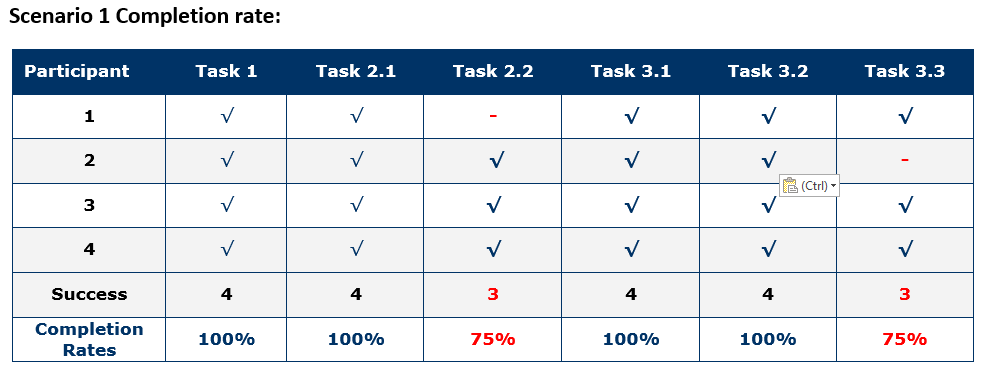
\includegraphics[width=\textwidth]{scenario1completionrate}
    \caption{Scenario 1 Completion Rate}
    \label{scenario1completionrate}
\end{figure}
\begin{figure}[h!]
    \centering
        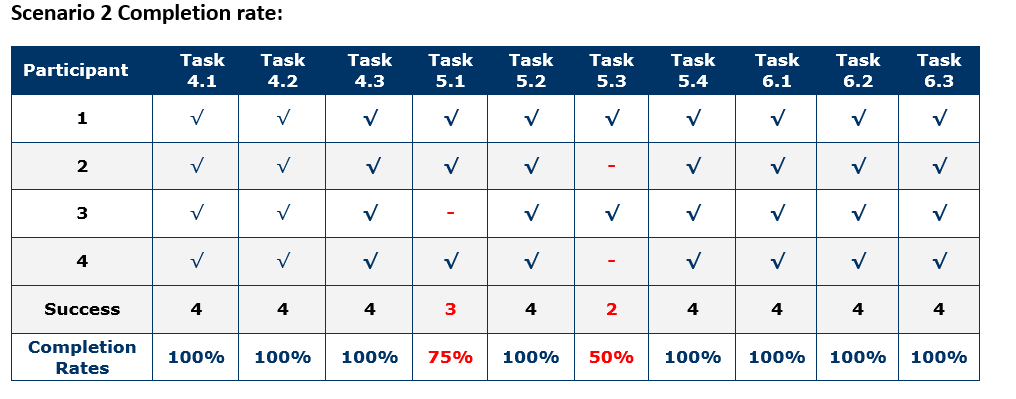
\includegraphics[width=\textwidth]{scenario2completionrate}
    \caption{Scenario 2 Completion Rate}
    \label{scenario2completionrate}
\end{figure}
All participants successfully completed (100\% Completion rate):
\begin{itemize}
	\item Task 1 - Start the application and set active repository. 
	\item Task 2.1 - View notifications. 
	\item Task 3.1 - Find the \emph{Reminder: Daily reflection} note and perform the daily summary. 
	\item Task 3.2 - Find and share the daily reflection note.
\end{itemize}
For Task 2.2(Find and archive congratulations notification) and 3.3(Find mood graph), 3 out of 4 participants completed the tasks(75\% Completion rate). \\

\textbf{Scenario 2 completion rates:}
All participants successfully completed (100\% Completion rate):
\begin{itemize}
	\item Task 4.1 - Create a team. 
	\item Task 4.2 - Set active team. 
	\item Task 4.3 - Identify team members. 
	\item Task 5.2 - Identify overdue milestones. 
	\item Task 5.4 - Find issue \#17
	\item Task 6.1 - Generate tag cloud
	\item Task 6.2 - Identify most used personal tags and team tags
	\item Task 6.3 - Find commit impact
\end{itemize}
3 out of 4 participants(75\%) successfully completed Task 5.1(Find all milestones for your repository), while 2 out 4(50\%) successfully completed Task 5.3 (Find your repositories issues). 

\subsubsection{Time on task}
Time on task for each participant was recorded. Some tasks were inherently more difficult to complete than others and is reflected by the average time on task.
\begin{figure}[h!]
    \centering
        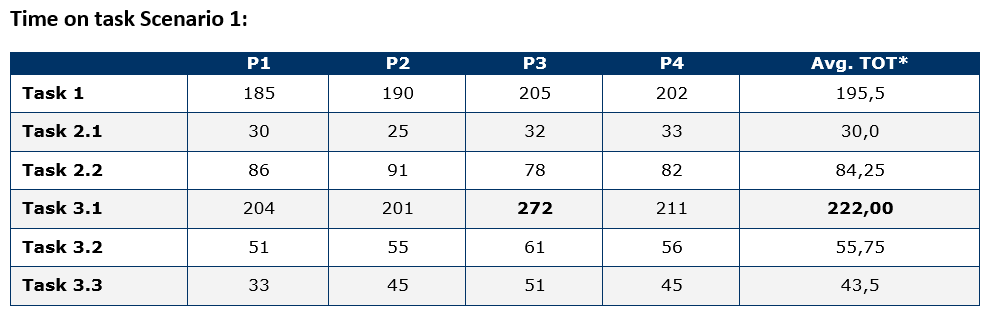
\includegraphics[width=\textwidth]{timeontaskscenario1}
    \caption{Time on task Scenario 1}
    \label{timeontaskscenario1}
\end{figure}
\begin{itemize}
	\item \textbf{Task 1(Start the application and set active team/repository)} showed a high average time on task. The main reason behind this was the authorization with GitHub which required users to login and authorize on the external GitHub.com page.
	\item \textbf{Task 2.1(View notifications)} showed a very similar time on task by the participants, the same can be seen on \textbf{Task 2.2(Find and archive notification)} although the time by each participant was over 80 seconds.
	\item \textbf{Task 3.1(Find reminder and perform daily reflection)} took the longest time to complete(average 222 seconds). However this was to be expected, as the daily reflection note requires participants to reflect on their work, and usually lasts for 2-5 minutes. This task also had the largest range in completion time, ranging from 204 seconds to 272 seconds. \textbf{Task 3.2(Find and share reflection note)} and \textbf{Task 3.3(Find mood graph)} participant time on task averaged 55 and 43 seconds. 
\end{itemize}
\begin{figure}[h!]
    \centering
        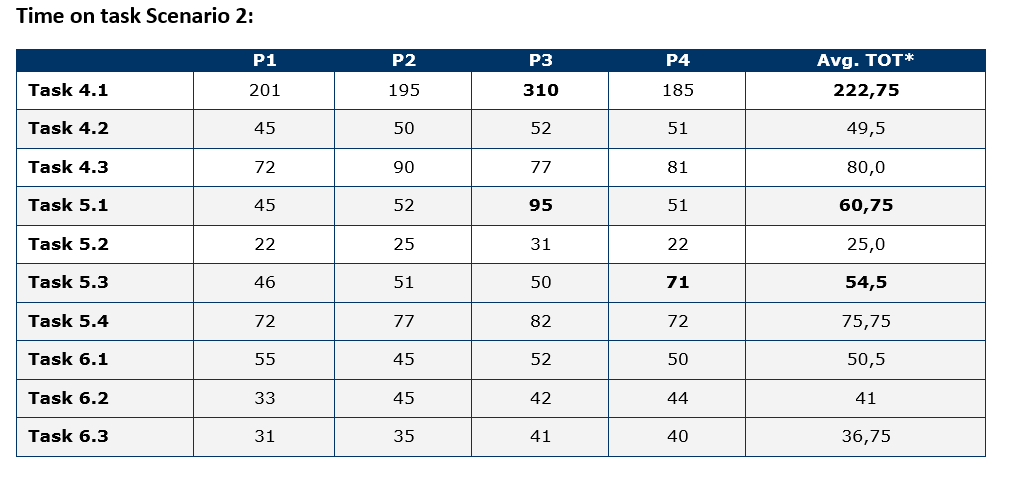
\includegraphics[width=\textwidth]{timeontaskscenario2}
    \caption{Time on task Scenario 2}
    \label{timeontaskscenario2}
\end{figure}
\begin{itemize}
	\item \textbf{Task 4.1(Create a team)} showed the longest completion time in Scenario 2. The main reason behind this was the amount of data that needed to be collected from GitHub and stored in the PeacefulBanana database. The task also showed the longest range in completion time, from 185 seconds to 310 seconds. The reason behind this large gap was mainly the difference in amount of data present in the GitHub repositories they chose to create a team for. \textbf{Task 4.2(Set active team) showed no major changes in completion time, and the same can be seen in \textbf{Task 4.3(Identify team members)}}
	\item \textbf{Task 5.1(Find all milestones)} showed that 3 out of 4 participants had very similar completion times(45, 52 and 51 seconds), but the average was increased by that the last participant had a completion time of 95 seconds. \textbf{Task 5.2(Identify overdue milestones)} showed very similar completion times, while \textbf{Task 5.3(Find repository issues)} had one participant at 71 seconds, while the rest used an average of 50 seconds. \textbf{Task 5.4(Find issue \#17)} showed an average of 75 seconds, with no significant differences. 
	\item \textbf{Task 6.1(Generate tag cloud)} averaged on 50 seconds, \textbf{Task 6.2(Identify most used individual and team tags)} averaged 41 seconds and \textbf{Task 6.3(Find commit impact)} averaged at 36 seconds, all with no significant difference in completion time. 
\end{itemize}
\subsubsection{Summary of Data}
The number of errors participants made while trying to complete the tasks were captured and recorded. Critical errors leads to participant failing in completing scenario, while non-critical errors is an error that does not prevent successful completion of the scenario. These errors along with task completions and time on task average for each task are represented in Figure \ref{datasummary}.
Low completion rate, occurrence of critical-errors and high time on task are highlighted in red. 
\begin{figure}[h!]
    \centering
        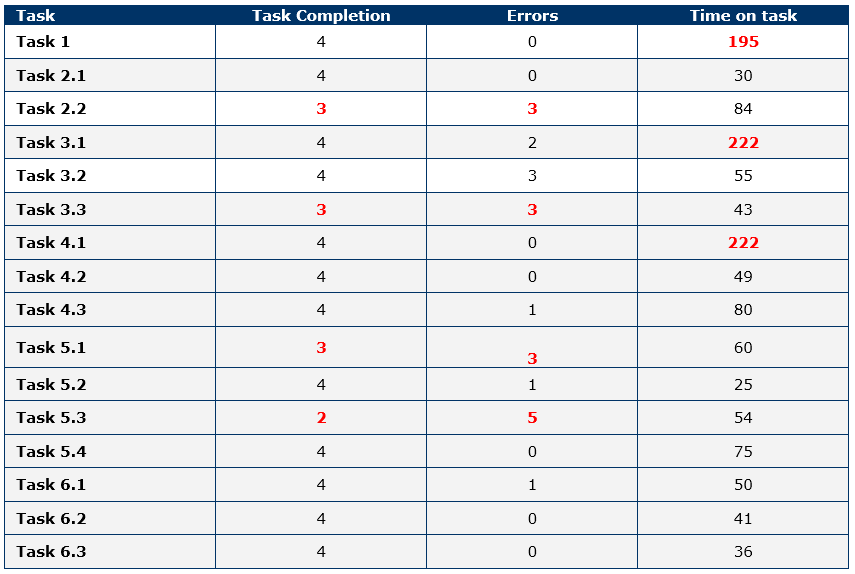
\includegraphics[width=\textwidth]{datasummary}
    \caption{Summary of Data}
    \label{datasummary}
\end{figure}

\subsubsection{Overall Metrics}
After completing the usability session, participants were given a \emph{System Usability Scale} form to answer\cite{brooke1996sus}. These can be seen in Figure: \ref{posttaskoverall}. \\

All participants agreed(i.e., agree or strongly agree) that they would use the application frequently and that the application was easy to use. All participants(100\%) also felt confident when using the application. The majority of the participants(75\%) felt the functions in the application were well integrated, and that most people would learn to use the system very quickly. Half of the participants(50\%) agreed that there were inconsistencies in the system. None of the participants(0\%) found the system unnecessarily complex or that it was cumbersome to use. Further none of the participants felt users would need support of a technical person to use the system(based on the intended user group) or that they needed to learn a lot before getting going with the system. The participants mentioned the quick start guide as a possible look-to document in case of trouble.  
\begin{figure}[h!]
    \centering
        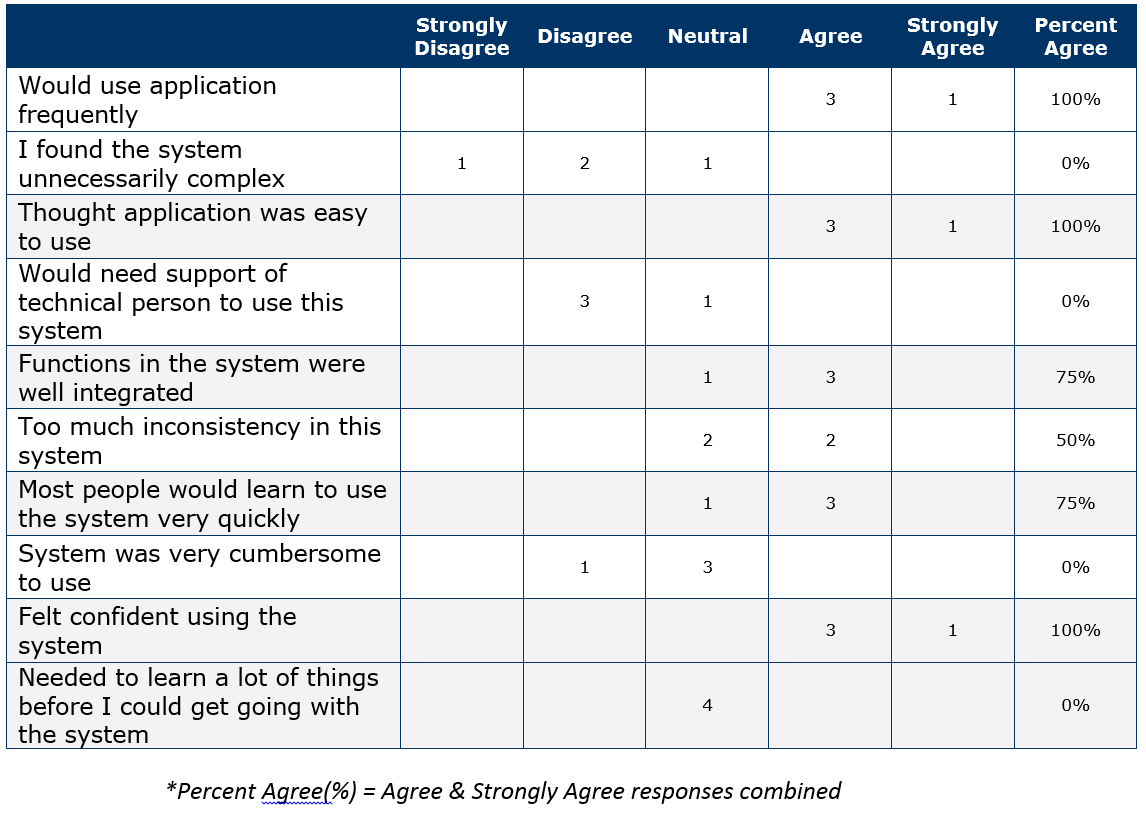
\includegraphics[width=\textwidth]{posttaskoverall}
    \caption{Post task}
    \label{posttaskoverall}
\end{figure}

\subsubsection{Reflection and sharing}
\label{subsubsec:reflection}
Participants were also asked to answer the questions identified in \ref{subsec:context}
\begin{itemize}
	\item Is the application easy to use, and can users achieve their goals in a timely manner?
\end{itemize}
Feedback here was that participants were satisfied with the ease of use as can be seen above, also time-on-task show that participants were mostly quite similar in the solving of tasks, and very few spikes. 
\begin{itemize}
	\item Identify the relationship users have with the aspect of reflection and sharing personal experiences.
\end{itemize}
On this context, participants answered that reflecting on their experiences is something they often do, but they don't collect them and thus forgets exactly what the experience was about. The application helped solve this problem by prompting and allowing users to reflect and then store it for later use. \\
When it comes to sharing, all participants were positive to this, although they strongly emphasized the need for an \emph{unshare} functionality. The missing ability to unshare these notes after hand could make them reluctant to share them in the first place, since when first shared it was always shared. One participant mentioned the possibility of letting notes be editable and share/unshareable for a specific time period, f.ex 24 hours, where afterwards they would be locked for editing.  
\begin{itemize}
	\item Does the tool present data in a way that triggers reflection for the user?
\end{itemize}
Participants responded that the tag-cloud and questions in the daily reflection note triggered them to reflect on experiences. Actually reading the questions in their mind, helped them to reflect on the experiences, instead of just having an empty text-field could lead to random thoughts being collected and not actually triggering reflection. The commit impact graph was mentioned as less-helpful as it didn't really justify the amount of work done. 
	
Participants also provided feedback for what they liked the most and least about the application, and recommendations for improving the application. \\
\subsubsection*{Most liked}
The participants liked the design of the application and that it was able to synchronize with their GitHub repositories automatically, without them having to worry about it. The personal tag-cloud and the ability to compare it directly with the team's tag cloud was also a joint feedback.
\subsubsection*{Least liked}
Participants commented that the way notifications were given was not optimal, and the registration process was a bit tedious.
\subsubsection{Recommendations}
In addition to the feedback gathered from section \ref{subsubsec:reflection} above this section provides recommended changes and justifications driven by the participant success rate, behaviors, and comments. The identified recommendations will improve the overall ease of use and address the areas where participants experienced problems or found the interface/information architecture unclear.
Feedback on recommendations on improvement was primarily to streamline the registration process. Also the participants commented that issues connected to a specific milestone, should be more visibly separated from issues connected to the whole repository. \\

\subsubsection*{Add unshare functionality}
\begin{figure}[h!]
    \centering
        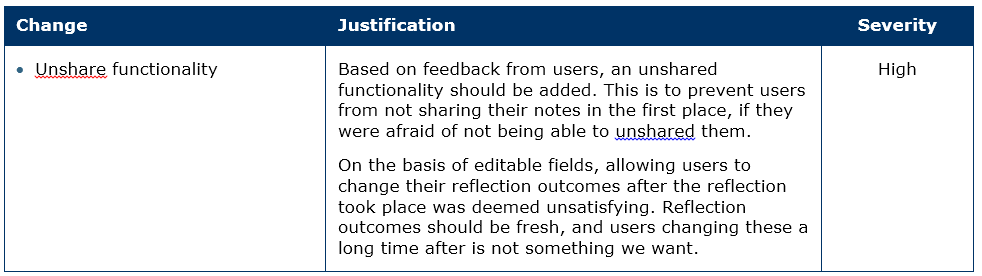
\includegraphics[width=\textwidth]{unshareimprovement}
    \caption{Adding unshare functionality to reflection notes.}
    \label{unshareimprovement}
\end{figure}

\subsubsection*{Remove commit impact}
\begin{figure}[h!]
    \centering
        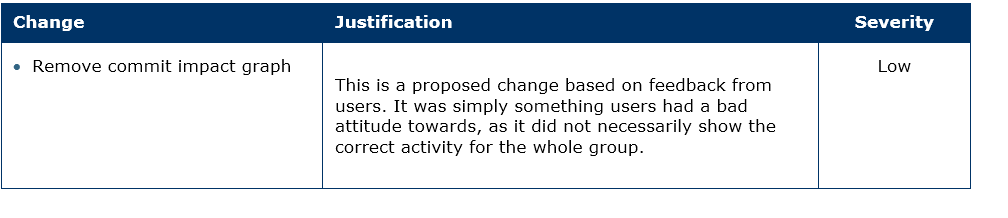
\includegraphics[width=\textwidth]{commitimprovement}
    \caption{Remove commit impact.}
    \label{commitimprovement}
\end{figure}

\subsubsection*{Task 1: Start application, login, link account with GitHub and set an active repository. } 
\begin{figure}[h!]
    \centering
        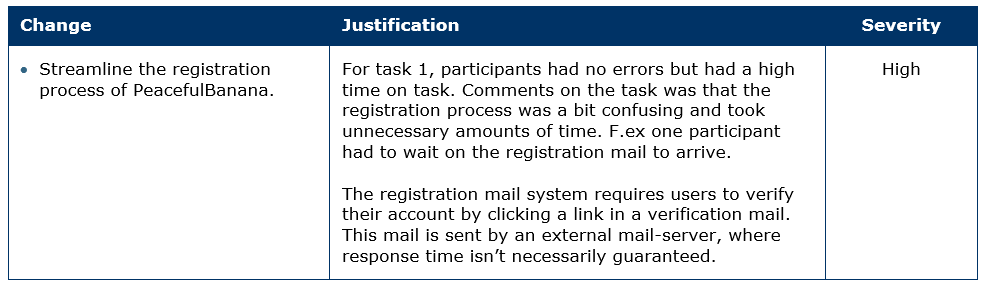
\includegraphics[width=\textwidth]{task1improvement}
    \caption{Task 1 changes and justification}
    \label{task1improvement}
\end{figure}
\subsubsection*{Task 2.2: Find the \emph{Congratulations} notification and archive it. Verify activation.}
\begin{figure}[H]
    \centering
        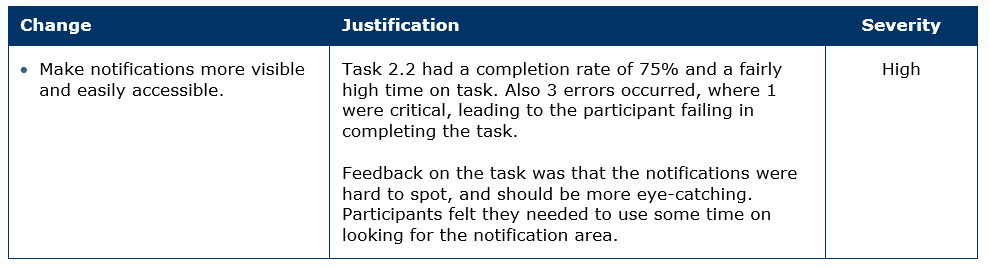
\includegraphics[width=\textwidth]{task22improvement}
    \caption{Task 2.2 changes and justification}
    \label{task22improvement}
\end{figure}
\subsubsection*{Task 3.3: Find the mood-graph.} 
\begin{figure}[h!]
    \centering
        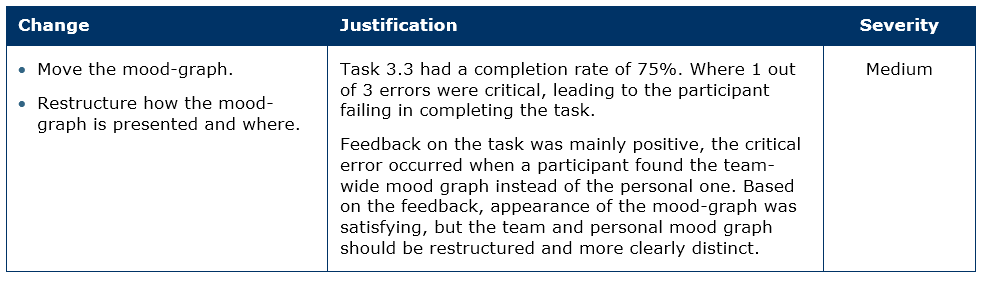
\includegraphics[width=\textwidth]{task33improvement}
    \caption{Task 3.3 changes and justification}
    \label{task33improvement}
\end{figure}
\subsubsection*{Task 5.1: Find all milestones for the current active repository.}
\begin{figure}[h!]
    \centering
        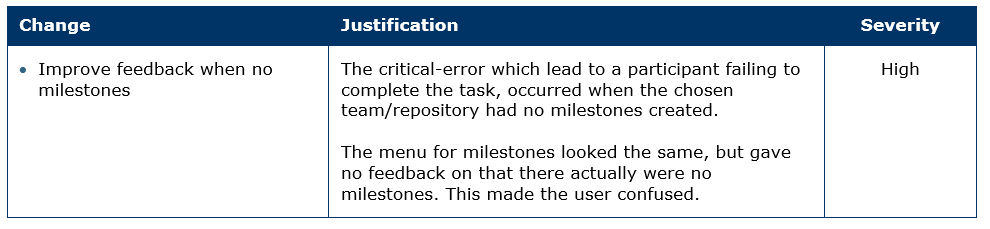
\includegraphics[width=\textwidth]{task51improvement}
    \caption{Task 5.1 changes and justification}
    \label{task51improvement}
\end{figure}
\subsubsection*{Task 5.3: Find repository related issues.} 
\begin{figure}[H]
    \centering
        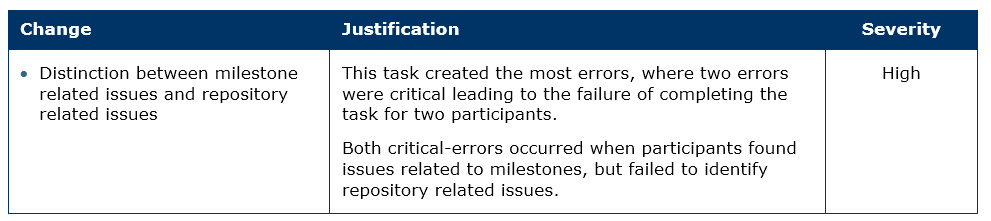
\includegraphics[width=\textwidth]{task53improvement}
    \caption{Task 5.3 changes and justification}
    \label{task53improvement}
\end{figure}

\subsection{Conclusion}
% Noe mer?
Most of the participants found the PeacefulBanana application to be well-organized, comprehensive, clean and uncluttered, very useful, and easy to use. Having an application to handle reflection in their daily work is to many if not all of the participants. Implementing the recommendations and further feedback from users will ensure a continued user-friendly application.

While some tasks had a high time-on-task, this was due to GitHub data collection, and is not something we have control over. It is a simple request to the GitHub API, which we need to receive before continuing. 
